\documentclass[portugues]{sobraep}
\titulo{Pulsar \\
          (Edição de Halloween)}


\author{Caleb Martim, Gabriel Henrique, Guilherme da Rocha\\
	\normalsize Bacharelado em Ciência da Computação\\
	\normalsize Univerisdade de Brasília\\
	\normalsize e-mail: autor1@email.br, autor2@email.com
}

\begin{document}

\maketitle

\begin{resumo}
	O objetivo deste documento é instruir os autores sobre a preparação dos trabalhos para publicação na Revista Eletrônica de Potência. Solicita-se aos autores que utilizem estas normas desde a elaboração da versão inicial até a versão final de seus trabalhos. Somente serão aceitos para publicação trabalhos que estejam integralmente de acordo com estas normas. Informações adicionais sobre procedimentos e normas podem ser obtidas também diretamente com o editor, ou, através do endereço eletrônico: https://mc04.manuscriptcentral.com/revistaep. Observa-se que são aceitas submissões em inglês, sendo que as normas para este idioma são apresentadas no mesmo endereço eletrônico. Este texto foi redigido segundo as normas aqui apresentadas para artigos submetidos em português.
\end{resumo}

\begin{palavraschave }
	Os autores devem apresentar um conjunto de até seis palavras-chave (em ordem alfabética, todas iniciais maiúsculas e separadas por vírgula) que possam identificar os principais tópicos abordados.
\end{palavraschave }

%~~~~~~~~~~~~~~~~~~~~~~~~~~~~~~~~~~~~~~~~
% Seções
%~~~~~~~~~~~~~~~~~~~~~~~~~~~~~~~~~~~~~~~~

% Introdução
\section{Introdução}

A Revista Eletrônica de Potência é um meio apropriado no qual os membros da SOBRAEP (Associação Brasileira de Eletrônica de Potência) e demais pesquisadores atuantes na grande área da Eletrônica de Potência podem apresentar e discutir suas atividades e contribuições científicas. Neste contexto, o Conselho Editorial convida os interessados a apresentarem artigos completos que envolvam o estado da arte na área, através de resultados teóricos e experimentais, além de informações tutoriais, nos tópicos de interesse da SOBRAEP. Caso o trabalho, ou parte dele, já tenha sido publicado em alguma revista ou conferência, nacional ou internacional, deve ser destacado no corpo do trabalho.

Serão aceitos trabalhos em português e inglês. Os textos submetidos em português devem conter também o título (title), resumo (abstract) e palavras-chave (keywords) em inglês, obrigatoriamente.

Os autores deverão submeter e acompanhar todo o processo de revisão e publicação através do https://mc04.manuscriptcentral.com/revistaep.

Somente serão aceitos trabalhos submetidos como documento em PDF editável (aberto). Portanto, após a edição de seu trabalho, em conformidade com estas normas, deverá ser gerado um documento em PDF com boa qualidade, para que possa ser submetido através do https://mc04.manuscriptcentral.com/revistaep. Observa-se ainda que para a publicação da versão final, somente serão aceitos artigos que estejam em conformidade com estas normas de edição e tenham preenchido o formulário \textit{Copyright} disponível no https://mc04.manuscriptcentral.com/revistaep.

A seção de Introdução tem o objetivo geral de apresentar a natureza do problema enfocado no trabalho, através de adequada revisão bibliográfica, o propósito e a contribuição do artigo submetido.

Caso seja pertinente, antes da Introdução pode ser incluída uma seção Nomenclatura com uma lista de variáveis usadas no texto. Este item não deve ser numerado, assim como os itens Agradecimentos, Referências e Dados Biográficos.

\subsection{Apresentação do Texto}

Os artigos submetidos para publicação na Revista Eletrônica de Potência devem possuir, preferencialmente, oito ou menos páginas. Artigos com um maior número de páginas deverão pagar uma taxa (R\$ 200,00 por página extra para autor correspondente membro da SOBRAEP ou R\$ 250,00 por página extra para autor correspondente não membro da SOBRAEP) antes da sua publicação, sendo aceitas até quatro páginas extras. Assim, o limite máximo é de 12 páginas.
A Revista Eletrônica de Potência é uma revista com acesso livre (open access), tendo as seguintes taxas de publicação: autor correspondente membro profissional da SOBRAEP grátis; autor correspondente membro estudante da SOBRAEP R\$ 65,00 por artigo; autor correspondente não membro da SOBRAEP R\$ 250,00 por artigo.

Deve-se usar, obrigatoriamente, as unidades do Sistema Internacional (SI ou MKS).

Cabe ao(s) autor(es) do trabalho a preparação dos originais e, posteriormente, seu envio de forma eletrônica, em PDF, através do https://mc04.manuscriptcentral.com/revistaep, de acordo com estas normas. Os trabalhos que estiverem fora dos padrões estabelecidos serão recusados, com a devida informação ao autor correspondente.

\subsection{Edição do Texto}

A editoração do trabalho deve ser feita selecionando o formato A4 (297 mm x 210 mm), de acordo com este exemplo.

Como processador de texto, estimula-se o uso do processador Word for Windows. Para envios em Latex apenas o editor Overleaf será aceito.

\subsubsection{Tamanho das letras utilizadas no trabalho}

Os tamanhos das letras especificadas nesta norma seguem o padrão do processador Word for Windows e o tipo de letra utilizado é Times New Roman. A Tabela I mostra os tamanhos padrões de letras utilizadas nas seções do artigo.

\begin{table}[H]
	\centering
	\caption{\textbf{Tamanhos e Tipos de Letras Utilizadas no Texto}}
	\footnotesize
	\setlength{\tabcolsep}{5pt}
	\begin{tabular}{cccc}
		\toprule [1.3pt]	
		\multicolumn{4}{c}{ \textbf{Estilo} } \\
		\hline
		\multirow{2}{1.1cm}{\centering \textbf{Tamanho (pontos)}} & \multirow{2}{*}{\textbf{Normal}} &
		\multirow{2}{*}{\textbf{Negrito}} & \multirow{2}{*}{\textbf{Itálico}} \\
		&  &  & \\		
		\hline
		8 & Texto de tabelas &  &  \\
		\hline
		\multirow{2}{*}{9} & \multirow{2}{2cm}{\centering Legendas de figuras}  &  &  \\
		& & & \\
		\hline
		\multirow{3}{*}{10} &
		\multirow{3}{2cm}{\centering Instituição dos autores; texto em geral; referências}  &
		\multirow{3}{2cm}{\centering Textos do resumo e palavras-chave; títulos de tabelas} &
		\multirow{3}{2.1cm}{\centering Títulos do resumo e palavras-chave} \\
		& &  &  \\
		& &  &  \\
		\hline
		\multirow{2}{*}{12} & \multirow{2}{2cm}{\centering Nomes dos autores}  & \multirow{2}{*}{Título em inglês} &  \\
		& & & \\
		\hline
		14 &  & Título do trabalho & \vspace*{-0.8mm}\\
		\bottomrule[1.3pt]
	\end{tabular} \label{table:TabelaI}
\end{table}

\subsubsection{Formatação das páginas}

Na formatação das páginas, as margens superior e inferior deverão ser fixadas em 25 mm, a margem esquerda em 18 mm e a margem direita em 12 mm. As colunas de textos deverão apresentar uma largura igual a 87 mm e um espaçamento entre si de 6 mm. A tabulação a ser utilizada na primeira linha dos parágrafos deverá ser fixada em 4 mm.

%Body Text
\section{Metodologia}

Neste item são apresentados os principais estilos utilizados para edição do trabalho.

\subsection{Organização Geral}

Os trabalhos a serem publicados na revista devem conter as seguintes seções principais: 1) Título; 2) Autores e Instituições de origem; 3) Resumo e Palavras-Chave; 4) Título em inglês (Title), Abstract e Keywords; 5) Introdução; 6) Corpo do trabalho; 7) Conclusões; 8) Referências; 9) Dados Biográficos. Esta ordem deve ser respeitada, a menos que os autores usem alguns itens adicionais, tais como: Nomenclatura; Apêndices e Agradecimentos.

A seguir serão feitos alguns comentários sobre os principais itens mencionados.

\subsubsection{Título}
O título em português do trabalho deve ser o mais sucinto possível, indicando claramente o assunto de que se trata. Deve estar centrado no topo da primeira página, sendo impresso em negrito, tamanho 14 pontos, com todas as letras em maiúsculo.

\subsubsection{Autores e instituições de origem}
Abaixo do título do trabalho (deixando uma linha em branco), também centrados na página, devem ser informados os nomes dos autores. Poderão ser abreviados os nomes e sobrenomes intermediários e escritos na sua forma completa o primeiro nome e o último sobrenome (letras do tipo 12 pontos). Imediatamente abaixo do nome dos autores, informar as instituições a que pertencem, cidade, estado e país e, logo abaixo, o endereço eletrônico de contato (letras do tipo 10 pontos).

\subsubsection{Resumo e palavras-chave}
Esta parte é considerada como uma das mais importantes do trabalho. É baseado nas informações contidas no resumo e nas palavras-chave que os trabalhos técnicos são indexados e armazenados em bancos de dados.

O resumo deve conter no máximo 200 palavras de forma a indicar as ideias principais apresentadas no texto, procedimentos e resultados obtidos. O resumo não deve ser confundido com uma introdução do trabalho e não deve conter abreviações, referências, figuras, etc. Na elaboração do resumo, como também em todo o trabalho, deve ser utilizada a forma impessoal como, por exemplo, ``... Os resultados experimentais mostraram que ...'' ao invés de ``...os resultados que nós obtivemos mostraram que...''. A palavra Resumo deve ser grafada em estilo itálico e em negrito. Já o texto deste Resumo será em estilo normal e em negrito.

Palavras-Chave são termos para indexação que possam identificar os principais tópicos abordados no trabalho. O termo Palavras-Chave deve ser grafado em estilo itálico e em negrito. Já o texto deste item será em estilo normal e em negrito.

\subsubsection{Informações em inglês}
O título deverá ser reproduzido em inglês, conforme normas apresentadas, destacando-se o estilo em letras todas maiúsculas, negrito e tamanho 12.

A palavra Abstract deve ser grafada em itálico e em negrito. Já o texto deste Abstract (em inglês) será em estilo normal e em negrito.

Keywords são termos para indexação, em inglês, que possam identificar os principais tópicos abordados no trabalho. O termo Keywords deve ser grafado em itálico e em negrito. Já o texto deste item será em estilo normal e em negrito.

\subsubsection{Introdução}
A introdução deve preparar o leitor para o trabalho propriamente dito, dando uma visão histórica do assunto, e servir como um guia a respeito de como o trabalho está organizado, enfatizando quais são as reais contribuições do mesmo em relação aos já apresentados na literatura. A introdução não deve ser uma repetição do Resumo e deve ser a primeira seção do trabalho a ser numerada como seção.

\subsubsection{Corpo do trabalho}
Os autores devem organizar o corpo do trabalho em diversas seções, as quais devem conter de forma clara, as informações a respeito do trabalho desenvolvido, facilitando a compreensão do mesmo por parte dos leitores.

\subsubsection{Conclusões}
As conclusões devem ser as mais claras possíveis, informando aos leitores sobre a importância do trabalho dentro do contexto em que se situa. As vantagens e desvantagens em relação aos já existentes na literatura devem ser comentadas, assim como os resultados obtidos e as possíveis aplicações práticas do trabalho.

\subsubsection{Referências}
As citações das referências ao longo do texto devem aparecer entre colchetes, antes da pontuação das sentenças nas quais estiverem inseridas. Devem ser utilizados somente os números das referências, evitando-se uso de citações do tipo ``...conforme referência [2]...''.

Os trabalhos que foram aceitos para publicação, mas que ainda não foram publicados, devem ser colocados nas referências com a citação ``no Prelo''.

Os artigos de periódicos e anais devem ser incluídos iniciando-se pelos nomes dos autores (iniciais seguidas do último sobrenome), seguido do título do trabalho, onde foi publicado (em itálico), número do volume, páginas, mês e ano da publicação.

No caso de livros, após os autores (iniciais seguidas do último sobrenome), o título deve ser em itálico, seguido da editora, da edição e do local e ano de publicação.

No final destas normas, é mostrado um exemplo de como devem ser apresentadas as referências~\cite{refbib1,refbib2,refbib3,refbib4,refbib5,refbib6,refbib7,refbib8}.

%\nocite{refbib1}
%\nocite{refbib2}
%\nocite{refbib3}
%\nocite{refbib4}
%\nocite{refbib5}
%\nocite{refbib6}
%\nocite{refbib7}
%\nocite{refbib8}

\subsubsection{Dados biográficos}
Os dados biográficos dos autores deverão estar na mesma ordem de autores colocados no início do trabalho e deverão conter basicamente os seguintes dados:
\begin{itemize}
	\item Nome Completo (em negrito e sublinhado);
	\item Local e ano de Graduação e Pós-Graduação;
	\item Experiência Profissional (Instituições e empresas em que já trabalhou, número de patentes obtidas, áreas de atuação, atividades científicas relevantes, sociedades científicas a que pertence, etc.). \newline
\end{itemize}

Caso sejam utilizados os itens adicionais Nomenclatura, Apêndices e Agradecimentos as seguintes instruções devem ser observadas:

\subsubsection{Nomenclatura}
A nomenclatura consiste na definição das variáveis e símbolos utilizados ao longo do trabalho. Não é obrigatória a sua inclusão e este item não é numerado como seção. Se este item for incluído, deve preceder o item Introdução. Caso os autores optem por não incluir este item, as definições das variáveis e símbolos utilizados devem ser incluídas ao longo do texto, logo após o seu aparecimento. No início destas normas é apresentado um exemplo para este item opcional.

\vspace*{-0.1mm}
\subsubsection{Agradecimentos e apêndices}
Os agradecimentos a eventuais colaboradores, assim como apêndices, não recebem numeração e devem ser colocados no texto, antes das referências.  No final deste trabalho  é mostrado um exemplo de como podem ser feitos estes agradecimentos.

Na última página do artigo os autores devem distribuir o conteúdo uniformemente, utilizando-se ambas as colunas, de tal forma que estejam paralelas quanto ao fechamento das mesmas.

\subsection{Organização das Seções do Trabalho}

A organização do trabalho em títulos e subtítulos serve para dividi-lo em seções, que ajudam o leitor a encontrar determinados assuntos de interesse dentro do trabalho. Também auxiliam os autores a desenvolverem de forma ordenada seu trabalho. O trabalho deve ser organizado em seções primárias, secundárias e terciárias.

As seções primárias são os títulos de seções propriamente ditos. São grafados em letras maiúsculas no centro da coluna, separadas por uma linha em branco anterior e uma posterior, e utilizam numeração romana e sequencial.

As seções secundárias são os subtítulos das seções. Apenas as primeiras letras das palavras que a compõe são grafadas em letra maiúscula, na margem esquerda da coluna sendo separada do resto do texto por uma linha em branco anterior. A designação das seções secundárias é feita com letras maiúsculas, seguidas de um ponto. Utilizam grafia em itálico.

As seções terciárias são subdivisões das seções secundárias. Apenas a primeira letra da primeira palavra que a compõe é grafada em letra maiúscula. A designação das seções terciárias é feita com algarismos arábicos, seguidos de um parêntese. Utilizam grafia em itálico.


\section{Resultados obtidos}

\subsection{Normas Editoriais}

Para artigos de autoria múltipla, é necessário informar a ordem de apresentação dos autores e preencher o Formulário \textit{Copyright} no https://mc04.manuscriptcentral.com/revistaep, autorizando a publicação do artigo. A Revista Eletrônica de Potência deve ser considerada fonte de publicação original. A Revista se reserva o direito de efetuar alterações de ordem normativa, ortográfica e gramatical nos arquivos originais, respeitando o estilo dos autores. As provas finais não serão enviadas aos autores. Os trabalhos publicados passam a ser de propriedade da Revista Eletrônica de Potência, ficando sua reimpressão total ou parcial sujeita à autorização expressa da SOBRAEP.

Figuras, tabelas e equações devem obedecer as normas apresentadas a seguir.

\subsection{Figuras e Tabelas}

As tabelas e figuras (desenhos ou reproduções fotográficas) devem ser inseridas no texto logo após serem citadas pela primeira vez, desde que caibam dentro dos limites da coluna; caso necessário, pode-se utilizar toda a área útil da página. A resolução das figuras deve ser superior a 300 dpi e, preferencialmente, no formato vetorial para boa qualidade de impressão. A legenda deve ser situada acima da tabela, enquanto que na figura deve ser colocada abaixo da mesma. As tabelas devem possuir títulos e são designadas pela palavra Tabela, sendo numeradas em algarismos romanos, sequencialmente. As legendas das tabelas devem estar centralizadas e em negrito.

As figuras necessitam de legenda, e são designadas pela palavra Figura no texto (Fig. na própria legenda), numeradas em algarismos arábicos, sequencialmente, com alinhamento justificado conforme exemplo. A designação das partes de uma figura é feita pelo acréscimo de letras minúsculas ao número da figura, começando pela letra a, como por exemplo, Figura 1(a).


\begin{figure}[H]
	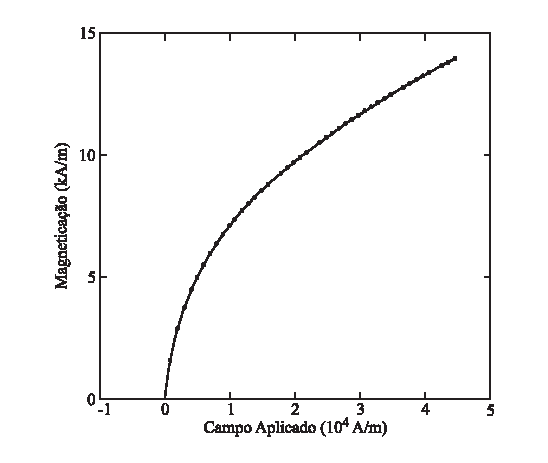
\includegraphics[scale=1]{figura.eps}
	\centering
	\caption{Curva de magnetização em função do campo aplicado. (Observe que o termo ``Fig.'' é abreviado. Existe um ponto após o número da figura, seguido de dois espaços antes da legenda).}
	\label{fig:fig1}
\end{figure}

Com o intuito de facilitar a compreensão dos gráficos, a definição dos eixos dos mesmos deve ser feita utilizando-se palavras e não letras, exceto no caso de formas de onda e planos de fase. As unidades devem ser expressas entre parênteses.~Por exemplo, utilize a denominação ``Magnetização (A/m)'', ao invés de ``M (A/m)''.

As figuras e tabelas devem ser posicionadas preferencialmente no início ou no final das colunas, evitando-as no meio das colunas. Devem ser evitadas tabelas e figuras, cujas dimensões ultrapassem as dimensões das colunas. As figuras devem ser preferencialmente editadas em preto, em fundo branco, uma vez que a versão impressa da revista não utiliza cores. Os traços devem ser de espessura tal que permitam uma impressão legível.
\balance
\subsection{Abreviações e Siglas}

As abreviações a serem utilizadas no texto, devem ser definidas na primeira vez em que aparecerem, como por exemplo, ``... Modulação por Largura de Pulso  (PWM)... ''.

\subsection{Equações}

A numeração das equações deve ser colocada entre parênteses, na margem direita, como em (1). As equações devem ser editadas de forma compacta e estar centralizadas na coluna. Caso a seção de nomenclatura não seja usada no início do texto, as variáveis devem ser definidas logo após as equações em que são indicadas, tal como:
\begin{equation}
	\Delta I_{L}=I_{o}+\frac{\sqrt{3}}{2}\frac{V_{i}}{Z}
\end{equation}
na qual:

\symboldescription{$\Delta I_{L}$}{corrente de piko no indutor ressonante;}
\symboldescription{$I_o$}{corrente de carga;}
\symboldescription{$V_i$}{tensão de alimentação;}
\symboldescription{$Z$}{impedância característica do circuito ressonante.}

\section{Conclusão}
Este artigo foi integralmente editado conforme as normas apresentadas para submissão de artigos em português.

\bibliographystyle{bib_sobraep}
\bibliography{referencias_sobraep}

\section*{Referências Bibliográficas}
\noindent\textbf{\underline{Fulano de Tal}}, nascido em 30/02/1960 em Talópoli, é engenheiro eletricista (1983), mestre (1985) e doutor em Engenharia Elétrica (1990) pela Universidade de Tallin.

Ele foi, de 1990 a 1995, coordenador do Laboratório de Tal. Atualmente é professor titular da Universidade de Tal. Suas áreas de interesse são: eletrônica de potência, qualidade do processamento da energia elétrica, sistemas de controle eletrônicos e acionamentos de máquinas elétricas.

Dr. Tal é membro da SOBRAEP, da SBA e do IEEE. Durante o período de 1998 a 2000 foi editor da revista Eletrônica de Potência da SOBRAEP.




\end{document}
